        \clearpage
        \begin{figure*}[ht]
            \pdfbookmark[2]{ID 05}{figure_id_05}
        	\centering
            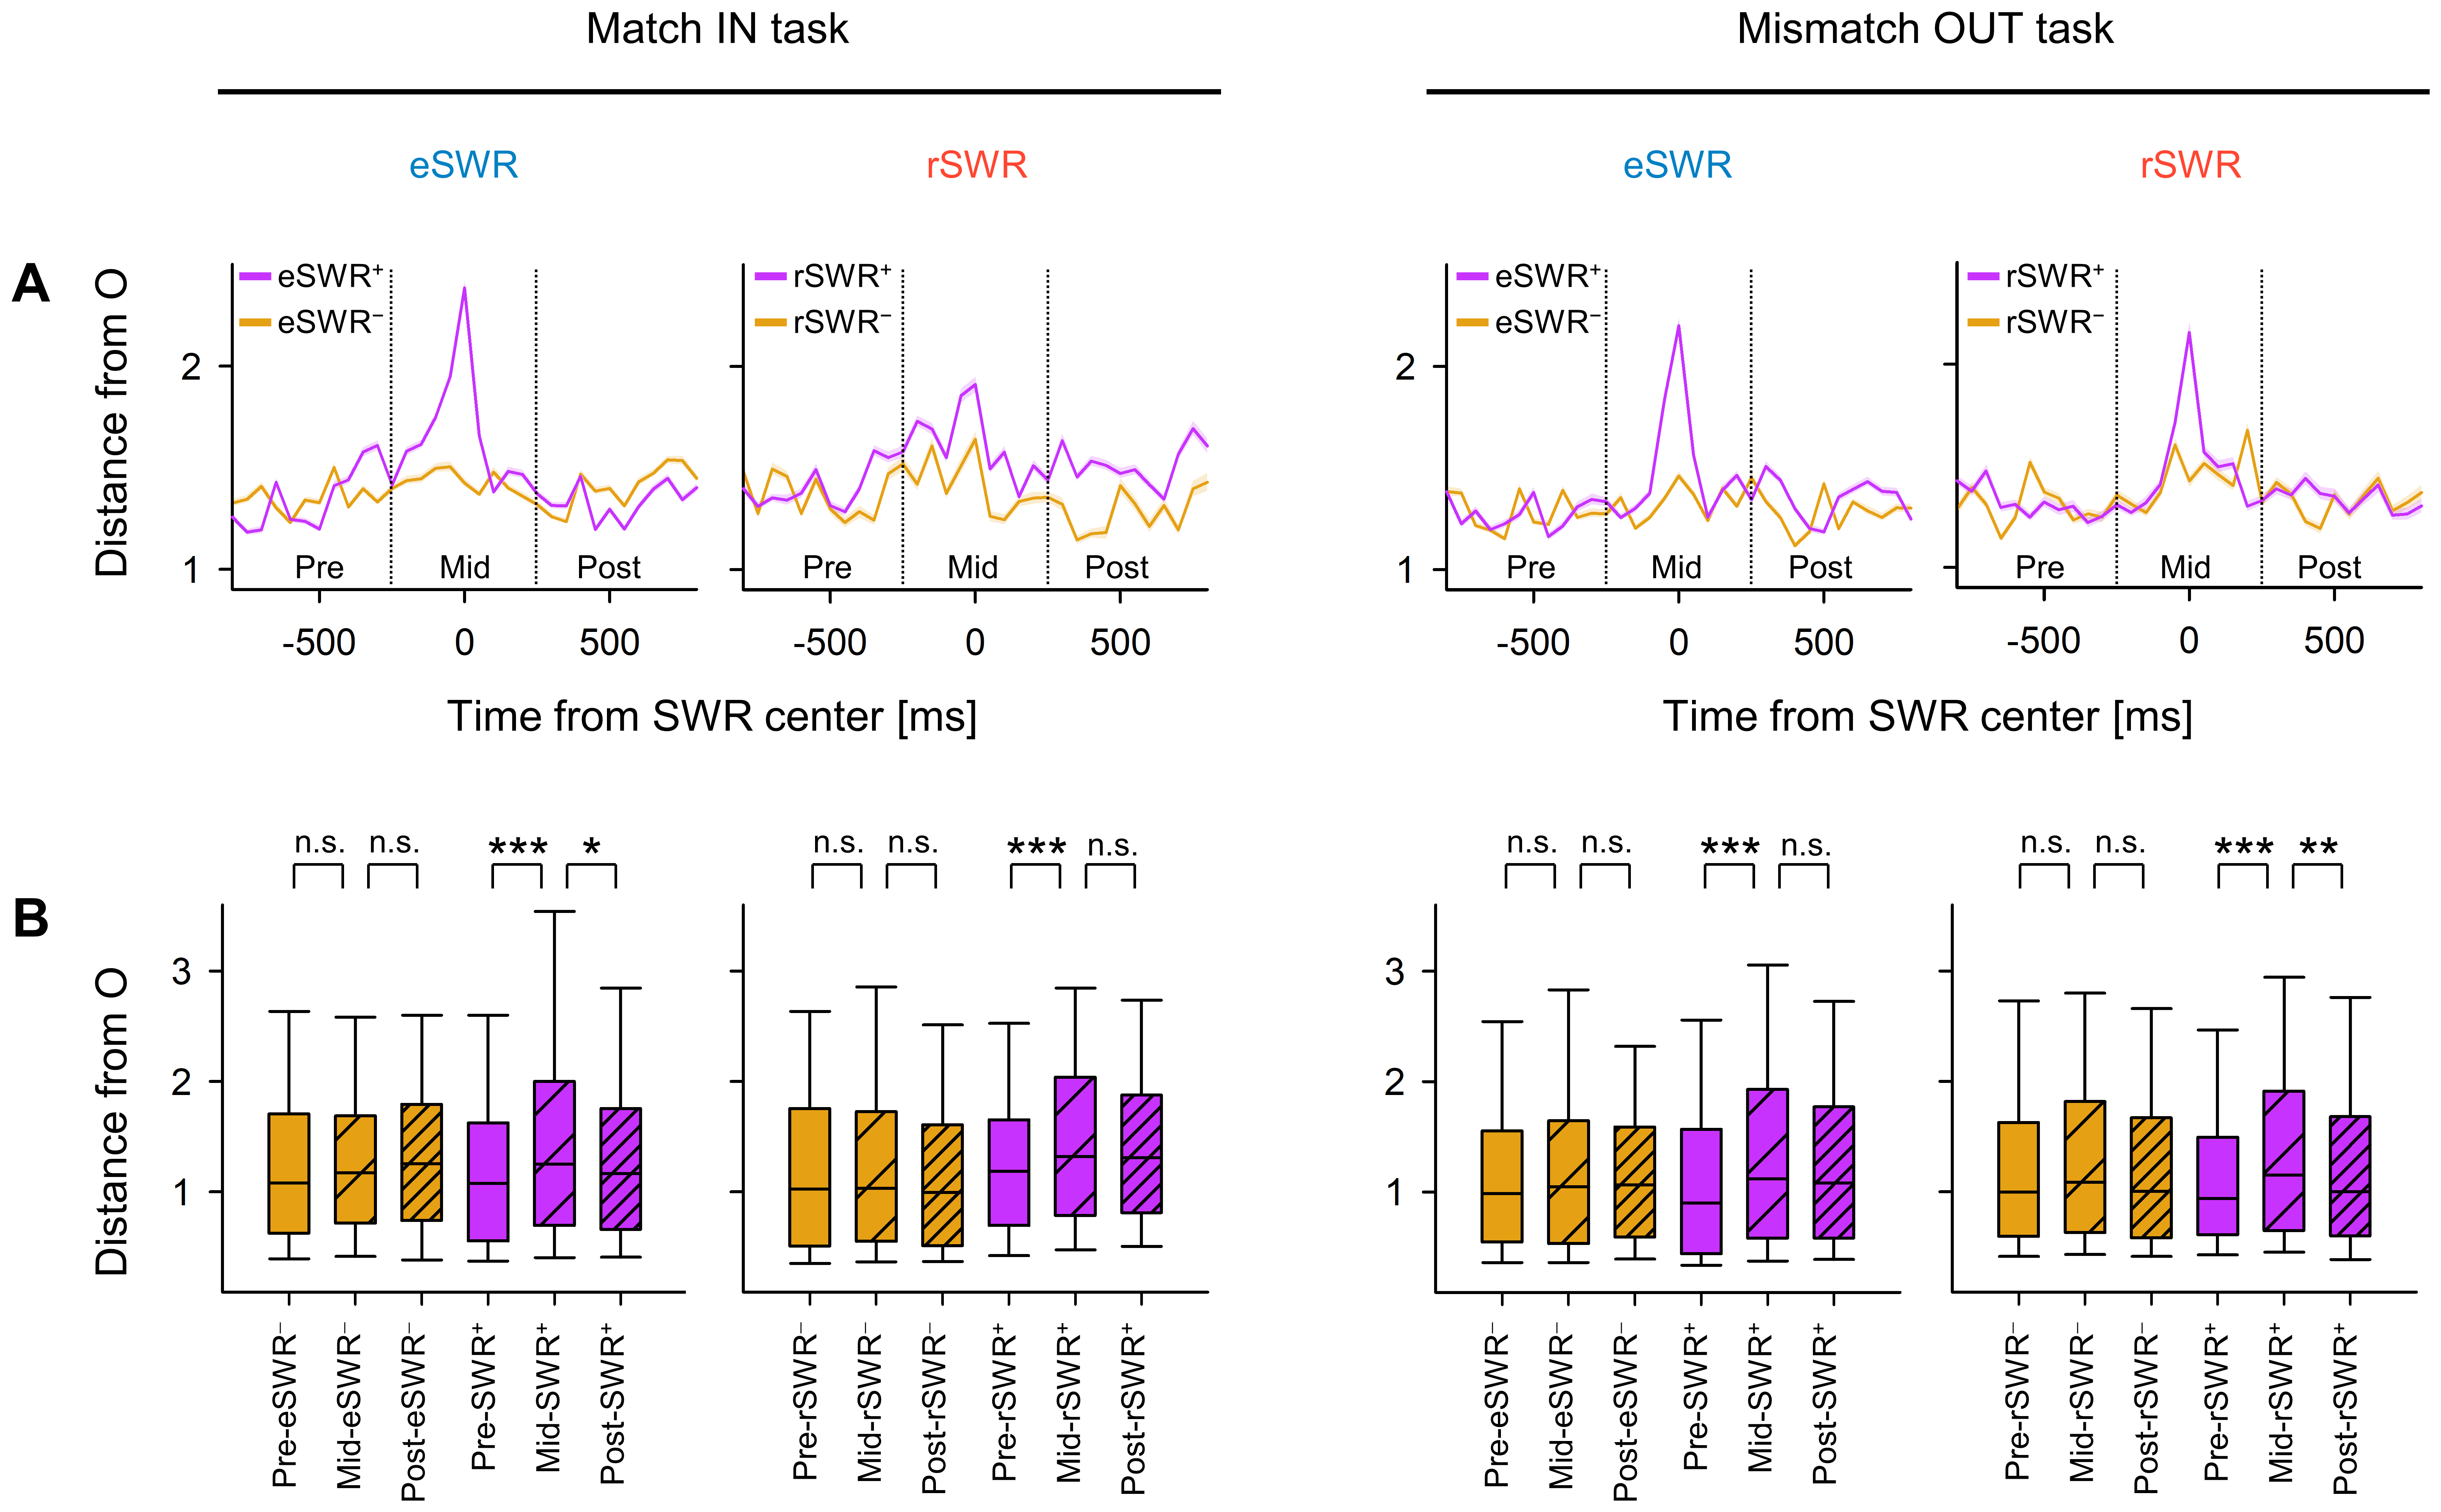
\includegraphics[width=1\textwidth]{./src/figures/.png/Figure_ID_05.png}
        	\caption{\textbf{
Transient Changes in Neural Trajectory During SWR Events
}
\smallskip
\\
\textbf{\textit{A.}} Depicted is the distance from the origin ($O$) of the peri-sharp-wave-ripple (SWR) trajectory, calculated as the mean \textpm 95\% confidence interval. The intervals might not be noticeable due to their narrow magnitudes. \textbf{\textit{B.}} Illustrated is the distance from the origin ($O$) during the pre-, mid-, and post-SWR phases (*\textit{p} $<$ 0.05, **\textit{p} $<$ 0.01, ***\textit{p} $<$ 0.001; evaluated using the Brunner--Munzel test). Abbreviations: SWR, sharp-wave ripple events; eSWR, SWR within the encoding phase; rSWR, SWR during retrieval phase; SWR$^+$, positive SWR event; SWR$^-$, control events for SWR$^+$; pre-, mid-, or post-SWR refer to the time intervals from $-800$ to $-250$ ms, from $-250$ to $+250$ ms, or from $+250$ to $+800$ ms, all in relation to the central point of the SWR.
}
% width=1\textwidth
        	\label{fig:05}
        \end{figure*}
